\section{Задача 1}

\subsection{Условие}

Найти неизвестную стационарную температуру границ двух сферических слоев из разных материалов. При этом на внутренней границе (отстоящей от центра) происходит теплообмен с внешней средой заданной температуры по закону Ньютона, а на внешней температура задана.

\subsection{Решение}

\begin{figure}[H]
    \begin{center}
        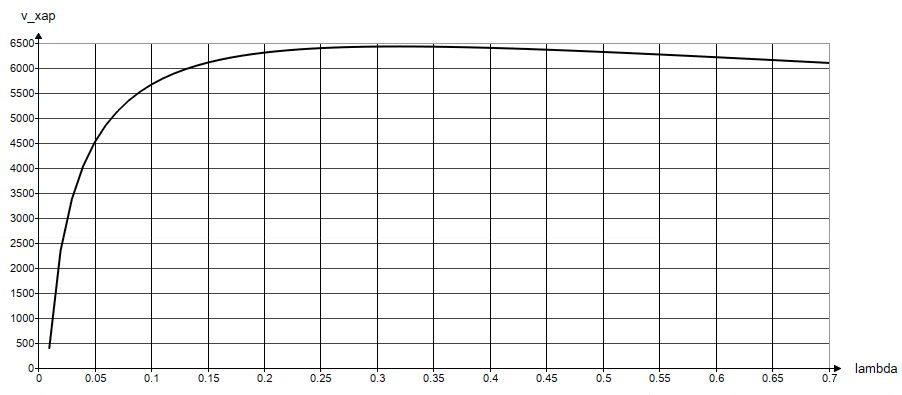
\includegraphics[width = 0.7\linewidth]{pic1.PNG}
        \caption{Условие задачи}
        \label{pic1}
    \end{center}
\end{figure}

Запишем основное уравнение теплопроводности:
\begin{equation}
    \label{eq1}
    \frac{\partial^2 U}{\partial t^2} = a^2 \Delta U
\end{equation}

Запишем общий вид граничных условий:
\begin{equation}
    \label{eq2}
    - \lambda \frac{\partial U}{\partial \vec{n}} \Big|_{r \in S} = \alpha \left( U \Big|_{r \in S} - U_\infty \right)
\end{equation}

Поскольку слоя сферические, запись уравнений будем вести в сферической системе координат. Также, поскольку задача стационарная, то левая часть уравнения (\ref{eq1}) равна нулю:
\begin{equation}
    \label{eq2.1}
    a^2 \Delta U = 0
\end{equation}

На внутренней поверхности теплообмен происходит по закону Ньютона:
\begin{equation}
    \label{eq3}
    - \lambda_1 \frac{\partial U_1}{\partial r} \Big|_{r = R_1} = \alpha (U_1 - U_1\Big|_{r = R_1})
\end{equation}

Запишем граничное условие для внешней поверхности:
\begin{equation}
    \label{eq3.1}
    U_2 \Big|_{r = R_\t{ст}} = U_2
\end{equation}

Запишем условие сопряжения:
\begin{equation}
    \label{eq4}
    U_1 \Big|_{r = R_\t{ст} - 0} = U_2 \Big|_{r = R_\t{ст} + 0}
\end{equation}

Запишем условие равенства мощностей тепловых потоков через границу раздела двух слоев:
\begin{equation}
    \label{eq4.1}
    \lambda_1 \frac{\partial U}{\partial r} \Big|_{r = R_\t{ст} - 0} = \lambda_2 \frac{\partial U}{\partial r} \Big|_{r = R_\t{ст} + 0}
\end{equation}

Запишем лапласиан для сферической системы координат:
\begin{equation}
    \label{eq5}
    \Delta = \frac{1}{r^2} \frac{\partial}{\partial r} \left( r^2 \frac{\partial}{\partial r} \right) + \frac{1}{r^2 \sin \theta} \frac{\partial}{\partial \theta} \left( \sin \theta \frac{\partial}{\partial \theta} \right) + \frac{1}{r^2 \sin \theta^2} \frac{\partial^2}{\partial \phi^2}
\end{equation}

Тогда распишем выражение (\ref{eq2.1}), используя (\ref{eq5}):
\begin{equation}
    \label{eq6}
    a^2 \left( \frac{1}{r^2} \frac{d}{dr} \left( r^2 \frac{dU}{dr} \right) \right) = 0
\end{equation}
\begin{equation}
    \label{eq7}
    \frac{d}{dr} \left( r^2 \frac{dU}{dr} \right) = 0
\end{equation}

Получили дифференциальное уравнение для обоих слоев. Решим его:
\begin{equation}
    \label{eq8}
    r^2 \frac{dU}{dr} = C' \;\;\; => \;\;\; \frac{dU}{dr} = \frac{C'}{r^2}
\end{equation}
\begin{equation}
    \label{eq9}
    U = -\frac{C'}{r} + C''
\end{equation}

Получим решения для двух участков:
\begin{itemize}
    \item Первый участок $R_1 \leq r \leq R_\t{ст}$:
    \begin{equation}
        \label{eq10}
        U_1 = - \frac{C_1}{r} + C_2
    \end{equation}
    \begin{equation}
        \label{eq10.1}
        \frac{dU_1}{dr} = \frac{C_1}{r^2}
    \end{equation}
    \item Второй участок $R_\t{ст} \leq r \leq R_2$:
    \begin{equation}
        \label{eq11}
        U_2 = - \frac{C_3}{r} + C_4
    \end{equation}
    \begin{equation}
        \label{eq12}
        \frac{dU_2}{dr} = \frac{C_3}{r^2}
    \end{equation}
\end{itemize}

Запишем условие сопряжения:
\begin{equation}
    \label{eq13}
    U_1(R_\t{ст}) = U_2(R_\t{ст}) = U_\t{ст}
\end{equation}
\begin{equation}
    \label{eq13.1}
    - \frac{C_1}{R_\t{ст}} + C_2 = - \frac{C_3}{R_\t{ст}} + C_4
\end{equation}

Запишем условие равенства мощностей тепловых потоков:
\begin{equation}
    \label{eq14}
    \lambda_1 \frac{dU_1}{dr} = \lambda_2 \frac{dU_2}{dr}
\end{equation}
\begin{equation}
    \label{eq15}
    \lambda_1 \frac{C_1}{R_\t{ст}^2} = \lambda_2 \frac{C_3}{R_\t{ст}^2}
\end{equation}

Используя (\ref{eq13.1}), (\ref{eq15}), (\ref{eq3.1}) и (\ref{eq3}) Получим систему уравнений для нахождения констант интегрирования:
\begin{equation}
    \label{eq16}
    \begin{cases}
        \displaystyle - \frac{C_1}{R_\t{ст}} + C_2 = - \frac{C_3}{R_\t{ст}} + C_4
        \\[10pt]
        \displaystyle \lambda_1 \frac{C_1}{R_\t{ст}^2} = \lambda_2 \frac{C_3}{R_\t{ст}^2}
        \\[10pt]
        \displaystyle - \frac{C_3}{R_2} + C_4 = U_2
        \\[10pt]
        \displaystyle - \lambda_1 \frac{C_1}{R_1^2} = \alpha \left( U_1 + \frac{C_1}{R_1} - C_2 \right)
    \end{cases}
\end{equation}

Из второго уравнения (\ref{eq16}) выразим $C_3$:
\begin{equation}
    \label{eq17}
    C_3 = \frac{C_1 \lambda_1}{\lambda_2}
\end{equation}

Из третьего уравнения (\ref{eq16}) выразим $C_4$:
\begin{equation}
    \label{eq18}
    C_4 = \frac{R_2 U_2 \lambda_2 + C_1 \lambda_1}{R_2 \lambda_2}
\end{equation}

Из первого уравнения (\ref{eq16}) выразим $C_2$:
\begin{equation}
    \label{eq19}
    C_2 = \frac{\left( R_2 R_\t{ст} U_2 + C_1 R_2 \right) \lambda_2 + \left( C_1 R_\t{ст} - C_1 R_2 \right) \lambda_1}{R_2 R_\t{ст} \lambda_2}
\end{equation}

Из четвертого уравнения (\ref{eq16}) выразим $C_1$:
\begin{equation}
    \label{eq20}
    C_1 = \frac{\left( R_1^2 R_2 R_\t{ст} U_2 - R_1^2 R_2 R_\t{ст} U_1 \right) \alpha \lambda_2}{\left( R_2 R_\t{ст} \lambda_1 + \left( R_1 R_2 R_\t{ст} + R_1^2 R_2 \right) \alpha \right) \lambda_2 + \left( R_1^2 R_2 - R_1^2 R_\t{ст} \right) \alpha \lambda_1}
\end{equation}

Тогда коэффициент $C_2$ равен:
\begin{equation}
    \label{eq21}
    C_2 = \frac{\left( R_2 R_\t{ст} U_2 \lambda_1 + \left( R_1 R_2 R_\t{ст} U_2 - R_1^2 R_2 U_1 \right) \alpha \right) \lambda_2 + \left( R_2 - R_\t{ст} \right) R_1^2 U_1 \alpha \lambda_1}{\left( R_2 R_\t{ст} \lambda_1 + \left( R_1 R_2 R_\t{ст} - R_1^2 R_2 \right) \alpha \right) \lambda_2 + \left( R_2 - R_\t{ст} \right) R_1^2 \alpha \lambda_1}
\end{equation}

Подставим полученные коэффициенты в выражение (\ref{eq10}) и найдем его значение при $r = R_\t{ст}$:
\begin{equation}
    \label{eq22}
    U_\t{ст} = U_1(R_\t{ст}) = \frac{R_1^2 \alpha \lambda_1 \left( R_\t{ст} - R_2 \right) \left( U_2 - U_1 \right)}{\left( R_2 R_\t{ст} \lambda_1 + \left( R_1 R_2 R_\t{ст} - R_1^2 R_2 \right) \alpha \right) \lambda_2 + \left( R_2 - R_\t{ст} \right) R_1^2 \alpha \lambda_1} + U_2
\end{equation}

\section{Задача 2}

\subsection{Условие}

Решить краевую задачу $U_t = aU_{xx}$ на промежутке $0 \leq x \leq l$, если $U_x(0, t) = 0$, $U_x(l, t) + \beta U(l, t) = 0$. Начальные условия $U(x, 0) = \phi(x)$.

\subsection{Решение}

Решим дифференциальное уравнение
\begin{equation}
    \label{eq23}
    \frac{\partial U}{\partial t} = a \frac{\partial^2 U}{\partial x^2}
\end{equation}

Воспользуемся методом разделения переменных Фурье:
\begin{equation}
    \label{eq24}
    U(x, t) = X(x) \cdot T(t)
\end{equation}

Подставим (\ref{eq24}) в (\ref{eq23}):
\begin{equation}
    \label{eq25}
    \frac{dT(t)}{dt} X(x) = a \frac{d^2 X(x)}{dx^2} T(t)
\end{equation}
\begin{equation}
    \label{eq26}
    \frac{dT(t)}{T(t) dt} \frac{1}{a} = \frac{1}{X(x)} \frac{dX^2(x)}{dx^2}
\end{equation}

Правая и левая часть (\ref{eq26}) не зависят друг от друга, поэтому по теореме Ляпунова их равенство достигается, когда левая и правая часть равны определенному числу:
\begin{equation}
    \label{eq27}
    \frac{dT(t)}{T(t) dt} \frac{1}{a} = \frac{1}{X(x)} \frac{dX^2(x)}{dx^2} = - \lambda^2
\end{equation}

Получили два независимых дифференциальных уравнения. Решим их:
\begin{equation}
    \label{eq28}
    \frac{dT(t)}{T(t) dt} \frac{1}{a} = - \lambda^2
\end{equation}
\begin{equation}
    \label{eq29}
    \frac{dT(t)}{T(t)} = - \lambda^2 a dt
\end{equation}
\begin{equation}
    \label{eq30}
    d \ln T(t) = - \lambda^2 a dt
\end{equation}
\begin{equation}
    \label{eq31}
    \ln T(t) = - \lambda^2 a t + C'
\end{equation}
\begin{equation}
    \label{eq32}
    T(t) = e^{- \lambda^2 a t + C'} = C e^{- \lambda^2 a t}
\end{equation}

Решим второе уравнение:
\begin{equation}
    \label{eq33}
    \frac{1}{X(x)} \frac{dX^2(x)}{dx^2} = - \lambda^2
\end{equation}
\begin{equation}
    \label{eq34}
    \frac{dX^2(x)}{dx^2} + \lambda^2 X(x) = 0
\end{equation}
\begin{equation}
    \label{eq35}
    X(x) = A \cos \lambda x + B \sin \lambda x
\end{equation}

Получим решение исходного дифференциального уравнения:
\begin{equation}
    \label{eq36}
    U(x, t) = (A \cos \lambda x + B \sin \lambda x)C e^{- \lambda^2 a t}
\end{equation}

Для нахождения констант интегрирования воспользуемся граничными и начальными условиями:
\begin{equation}
    \label{eq37}
    \frac{\partial U}{\partial x}(0, t) = 0
\end{equation}

Из (\ref{eq36}) получим:
\begin{equation}
    \label{eq38}
    \frac{\partial U}{\partial x}(x, t) = \left( B \lambda \cos \lambda x - A \lambda \sin \lambda x \right) T(t)
\end{equation}

Подставим (\ref{eq38}) в (\ref{eq37}):
\begin{equation}
    \label{eq39}
    B \lambda T(t) = 0
\end{equation}
\begin{equation}
    \label{eq40}
    B = 0
\end{equation}

Получим:
\begin{equation}
    \label{eq41}
    U(x, t) = A C \cos \lambda x \cdot e^{- \lambda^2 a t}
\end{equation}

Переобозначим константу:
\begin{equation}
    \label{eq42}
    D = AC
\end{equation}
\begin{equation}
    \label{eq43}
    U(x, t) = D \cos \lambda x \cdot e^{- \lambda^2 a t}
\end{equation}

Второе граничное условие:
\begin{equation}
    \label{eq44}
    \frac{\partial U}{\partial x} (l, t) + \beta U(l, t) = 0
\end{equation}
\begin{equation}
    \label{eq45}
    \frac{\partial U}{\partial x} (x, t) = - D \lambda \sin \lambda x \cdot T(t)
\end{equation}

Подставим (\ref{eq45}) в (\ref{eq44}):
\begin{equation}
    \label{eq46}
    - D \lambda \sin \lambda l \cdot T(t) + \beta D \cos \lambda l T(t) = 0
\end{equation}
\begin{equation}
    \label{eq47}
    \lambda \sin \lambda l = \beta \cos \lambda l
\end{equation}
\begin{equation}
    \label{eq48}
    \tg \lambda l = \frac{\beta}{\lambda}
\end{equation}

Значения $\lambda$ должны удовлетворять выражению (\ref{eq48}). Поскольку таких значений бесконечно много можно воспользоваться свойством, что линейная комбинация решений дифференциального уравнения также является решением этого уравнения:
\begin{equation}
    \label{eq49}
    U(x, t) = \sum_{n = 0}^{\infty} D_n \cos \lambda_n x \cdot e^{- \lambda_n^2 a t}
\end{equation}

Воспользуеся начальным условием:
\begin{equation}
    \label{eq50}
    U(x, 0) = \phi (x)
\end{equation}

Для нахождения коэффициентов $D_n$ разложим функцию $\phi (x)$ в ряд по собственным функциям:
\begin{equation}
    \label{eq51}
    \phi (x) = \sum_{n = 0}^{\infty} \Gamma_n \cos \lambda_n x
\end{equation}
\begin{equation}
    \label{eq52}
    \Gamma_n = \frac{2}{l} \int_{0}^{l} \phi(x) \cos \lambda_n x dx
\end{equation}

Подставим (\ref{eq51}) и (\ref{eq49}) в (\ref{eq50}):
\begin{equation}
    \label{eq53}
    \sum_{n = 0}^{\infty} D_n \cos \lambda_n x = \sum_{n = 0}^{\infty} \Gamma_n \cos \lambda_n x
\end{equation}

Воспользуемся свойством ортогональности собственных функций:
\begin{equation}
    \label{eq54}
    D_n = \Gamma_n = \frac{2}{l} \int_{0}^{l} \phi(x) \cos \lambda_n x dx
\end{equation}

Получим итоговое решение краевой задачи:
\begin{equation}
    \label{eq55}
    U(x, t) = \sum_{n = 0}^{\infty} \left[ \left( \frac{2}{l} \int_{0}^{l} \phi(x) \cos \lambda_n x dx \right) \cos \lambda_n x \cdot e^{- \lambda_n^2 a t} \right]
\end{equation}